\documentclass{article}

\usepackage{hyperref}
\usepackage{ctex}
\usepackage{indentfirst}
\usepackage{booktabs}
\usepackage{graphicx}
\graphicspath{{picture/},{pics/}}

\title{\heiti 海洋微塑料的危害和处理}
\author{贾沫晗 U202315338 自卓2301班}
%\date{\today}								

\usepackage{geometry}												
\geometry{left=3.2cm,right=3.2cm,top=3.8cm,bottom=3.8cm}			% 设置页边距
\usepackage{fancyhdr}												% 设置页眉
\pagestyle{fancy}	
\fancyhf{}
\cfoot{\thepage}													% 设置页码
\renewcommand{\sectionmark}[1]{\markboth{第\thesection 章\quad 		% 设置页眉内容为章标题
		\ #1}{}}


\begin{document}
	\maketitle
	\tableofcontents
	
	%\textrm{Roman Family}
	%\rmfamily Roman Family
	%\textmd{Medium Series} \textbf{Boldface Series}
	%\textup{Upright Shape} \textit{Italic Shape}
	%\textsl{Slanted Shape} \textsc{Small Caps Shape}
	\begin{abstract}
		\textbf{ 摘要:} 近年来,环境污染问题日益严重,海洋污染也不可忽视。其中,海洋微塑料具有很大的危害,对海洋生态系统和人类健康造成了严重威胁。如何有效处理海洋微塑料成为一个至关重要的问题。本文通过文献综述和资料查找,概述了海洋微塑料的危害和处理方法。目前,常用的处理方法包括物理方法、化学方法和生物方法。物理方法包括过滤、离心和膜分离等,能够有效去除海洋微塑料;化学方法主要利用化学反应将微塑料分解为无害物质;生物方法则利用微生物降解微塑料,是一种环保和可持续的处理方式。
		
		\textbf{关键词:} 海洋微塑料,毒性效应,微塑料污染,国际合作
	\end{abstract}

    
    
    \section{引言} 海洋微塑料是指直径小于5毫米的塑料颗粒,广泛分布于海洋环境中。随着全球塑料消费量的增加和塑料废弃物的不当处理,海洋微塑料污染问题日益严重。这些微塑料颗粒对海洋生态系统和人类健康构成了重大威胁,已引起全球关注。海洋微塑料的主要来源包括塑料垃圾的直接排放、塑料制品的磨损以及海上运输活动。不当处理塑料垃圾导致大量塑料进入海洋,而塑料制品的磨损会释放出微小的塑料颗粒。此外,海上运输活动也是微塑料的重要来源。这些微塑料颗粒在海洋中长期存在,被海洋生物误食,进而进入食物链,对海洋生态系统产生负面影响。海洋微塑料不仅破坏海洋生态系统,也对人类健康构成潜在风险。研究表明,微塑料颗粒可以通过食物链传递到人类体内,可能对健康产生不利影响。此外,海洋微塑料还可能通过水源进入人类饮用水系统,增加人类暴露于微塑料的风险。因此,寻找有效的海洋微塑料处理方法至关重要。目前,物理、化学和生物方法在海洋微塑料处理上被广泛研究和应用。物理方法包括过滤、离心和膜分离等,能够有效去除海洋微塑料;化学方法则利用化学反应将微塑料分解为无害物质;生物方法利用微生物降解微塑料,是一种环保和可持续的处理方式。本文旨在综述海洋微塑料的危害及其处理方法和技术,通过深入研究和分析不同的处理方法,为解决海洋微塑料污染问题提供科学依据和技术支持。此外,政府、科研机构和企业应加强合作,共同推动海洋微塑料处理技术的研发和应用。公众教育和法律法规的制定也是解决海洋微塑料问题的重要手段。只有综合应用各种方法和措施,才能有效减少海洋微塑料污染,保护海洋生态环境和人类健康。

    \section{海洋微塑料的来源及其形成过程}
    
    海洋微塑料的主要来源包括以下几个方面:
    
    \subsection{塑料垃圾的直接排放}塑料垃圾的直接排放:塑料制品的使用量巨大,大多数塑料制品在使用后被丢弃,其中一部分被直接排入海洋。据JAMBECK J R\cite{01}等人的研究计算,2010年全球192个沿海国家产生了2.75亿吨(MT)的塑料垃圾,其中有480万至1270万吨进入了海洋。根据图1, 2011年至2015年,我国近海地区的海洋垃圾(包括漂浮垃圾和海滩垃圾)中,塑料垃圾的比例始终超过70\%,且比例逐年上升,凸显了海洋塑料垃圾处理问题的日益严峻。
    \begin{figure*}
    	\centering
    	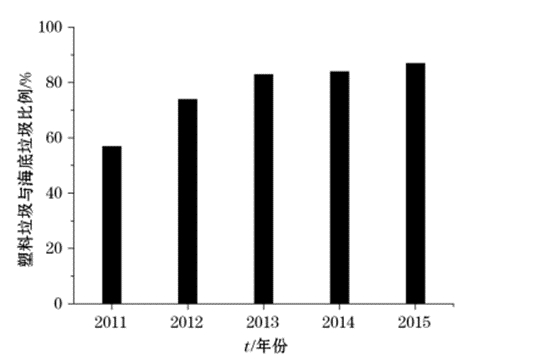
\includegraphics{data}
    	\caption{2011—2015年我国近海海底垃圾中塑料垃圾的比例\cite{02}}
    	\label{fg:state}
    \end{figure*}
       %{ 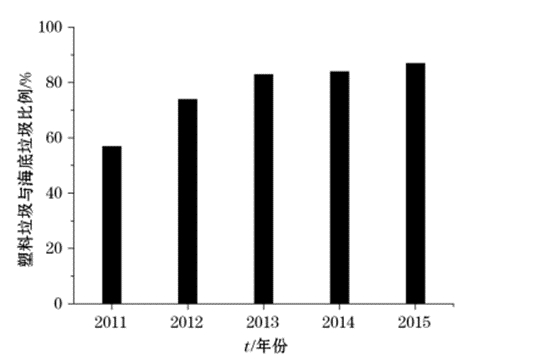
\includegraphics{data}}
     
    \subsection{塑料制品的磨损} 塑料制品的磨损:在长期使用过程中,塑料制品会因磨损而释放出微小的塑料颗粒。例如,合成纤维制成的衣物在洗衣机洗涤过程中会释放出微塑料纤维,这些纤维通过污水系统最终进入海洋。
    
    \subsection{塑料微珠的使用} 塑料微珠的使用:塑料微珠是一种广泛存在的塑料微粒,常见于个人护理产品、清洁剂和化妆品中,如洗面奶、牙膏和沐浴露等。使用这些产品后,微珠会随废水流入下水道,最终流入海洋。
    
    \subsection{农业和工业排放} 农业和工业排放:农业和工业活动也是海洋微塑料的重要来源。农业中使用的塑料农膜、农药容器和肥料袋等,及工业中产生的塑料包装材料和废弃物,都可能通过排放或流失进入水体,最终汇入海洋。
    
    \subsection{海洋运输活动} 海洋运输活动:海洋运输是全球贸易的重要环节,但它也是海洋微塑料的一个重要来源。船舶废弃物、货物包装材料以及船舶燃料中的塑料颗粒都有可能流入海洋。
    
    这些来源导致海洋中存在大量的微塑料颗粒,它们被海流和风力分散到各个区域,在各个港口及海域都有广泛分布,如表1所示,对海洋生态系统和生物多样性造成了严重影响。


    %\includegraphics{1512qb00448_10_01600}
        \begin{center} 
        \begin{tabular}{p{5cm} p{3cm} p{3.2cm}}
    	   \hline
    	   调查区域 & 粒径 & 塑料丰富度\\
    	   \hline
    	   奥地利多瑙河&<20mm & 0.32±4.67个/m$^{3}$\\
    	   英格兰西南部的泰马河口 & >5mm & 0.03个/m$^{3}$\\
    	   巴西戈亚纳河口 & <5mm& 0.26个/m$^{3}$\\
    	   地中海科西嘉岛卡尔维湾 &0.2~10mm &0.06个/m$^{3}$\\
    	   地中海科西嘉岛卡尔维湾 & >10mm & 0.01个/m$^{3}$\\
    	   北海南部的翡翠湾 & <5mm& 64±194个/L\\
    	   加拿大夏洛特皇后湾 &  398±376 μm &7630±1410个/ m$^{3}$\\
    	   加拿大乔治亚海峡 & 513±494 μm &3210±628个/m$^{3}$\\
    	   英吉利海峡西部&<5mm&0.27个/m$^{3}$\\
    	   地中海西北部&0.3~5mm &0.12个/m$^{3}$\\
    	   意大利撒丁岛西海域&<5 mm&0.15个/m$^{3}$\\
    	   利古里亚海和撒丁岛海域&<5 mm&0~10个/m$^{3}$\\
    	   葡萄牙海岸&<5 mm&0.002~0.036个/m$^{3}$\\
    	   加拿大温哥华岛西海岸&558±521 μm&1710±1110个/m$^{3}$\\
    	   韩国南部海岸& 总含量 & 211±117个/L\\
    	   韩国南部海岸&<50μm&103±59个/L\\
    	   韩国南部海岸&50~100μm&69±41个/L\\
    	   韩国南部海岸&100~200μm&23±20个/L\\
    	   韩国南部海岸&200~500μm&11±11个/L\\
    	   韩国南部海岸&500~1000μm&2.9±3.4个/L\\
    	   韩国南部海岸&>1000μm&2.1±2.9个/L\\
    	   中国长江口&0.5~5mm&4137.3±2461.5个/m$^{3}$\\
    	   中国东海海岸&0.5~5mm&0.167±0.138个/m$^{3}$\\
    	   \hline
        \end{tabular}
      \end{center}  
        
      \begin{center}
          表1:\quad 全球海岸区域海面漂浮微塑料的粒径和丰度\cite{03}
      \end{center}  
      
        
    \section{海洋微塑料的危害}
    
    \subsection{对海洋生态系统的破坏}对海洋生态系统的破坏:海洋微塑料对海洋生态系统造成了严重的破坏。微塑料颗粒可能被海洋生物误食,从而影响它们的生长、繁殖和生存能力。此外,这些颗粒还可能堵塞海洋生物的消化道,干扰营养吸收和能量转化,进而对整个海洋食物链产生连锁反应,破坏海洋生态系统的平衡与稳定。根据ALLSOPP \cite{04}等人的研究表明,至少有267种不同的物种遭受了海洋废弃物的缠绕或摄入,包括海鸟、海龟、海豹、海狮、鲸鱼和鱼类。同时,塑料碎片在全球范围内广泛分布,从极地地区到赤道,污染了所有的海洋环境。
    
    \subsection{毒性效应} 毒性效应:微塑料中的化学物质和添加剂可能释放出毒性物质,给海洋生物带来严重的毒性效应。这些毒性物质不仅可以干扰生物的生理过程,损害细胞和组织,甚至可能导致生物的死亡。除此之外,海洋微塑料还可能引发复合化学污染的问题。微塑料中的有毒单体添加剂以及从环境中富集的持久性有机污染物和重金属等\cite{05}。会对海洋生物造成进一步的伤害。微塑料和纳米塑料颗粒可以被许多海洋生物摄取,并在生物体内积累。这些颗粒可以通过食物链逐级富集到更高等的生物体中,进而影响它们的正常新陈代谢和繁殖。特别是尺寸较小的纳米塑料颗粒更容易进入细胞和组织,且其表面带有正电荷的纳米塑料颗粒对细胞生理活动的影响尤为明显。微塑料和纳米塑料中的添加剂及其表面吸附的污染物在生物体内释放时,其对生物体的危害远远超过了微塑料颗粒本身的影响\cite{06}。刘强\cite{07}的研究表明,海洋微塑料的毒性效应不仅包括致死效应、生长发育毒性、行为毒性、生殖毒性、免疫毒性以及基因与遗传毒性,还包括微塑料与其他污染物的复合毒性。当微塑料颗粒与其他污染物通过吸附或表面反应作用结合在一起时,这些污染物可以成为进入生物组织和器官的载体,从而使微塑料与化学污染物共同对生物体产生复合毒性效应。
    
    \subsection{食物链传递} 食物链传递:微塑料通过食物链传递到海洋生物体内,最终有可能进入人类的食物链。当人类摄入受污染的海产品时,微塑料颗粒可能进入体内,带来潜在的健康风险。研究表明,微塑料可能对人体的消化系统、免疫系统和内分泌系统产生不良影响,并可能引发慢性疾病,如癌症和神经系统疾病。
    
    \subsection{水源污染} 水源污染:海洋微塑料还可能通过水源进入人类饮用水中,从而增加了人类暴露于微塑料的风险。微塑料颗粒可能穿过水处理系统的过滤器,进入自来水供应中。长期饮用这种受污染的水源可能对人体健康产生潜在的不良影响。
    
    \subsection{人类社会经济}人类社会经济:2014-06在首届联合国环境大会上,UNEP发布的《UNEP Year Book 2014》和《Valuing Plastic》两项报告中指出,海 洋中大量塑料垃圾对海洋生物生存的威胁日益加剧,保守估计每年给海洋生态系统造成的经济损失高达130亿美元\cite{02}。
    可以看到,海洋微生物对海洋生态系统、水源、人类社会等都产生了很大的危害,处理海洋微塑料不可等待,以下将列出处理海洋微生物的多种科学方法。
    
    
    \section{海洋微塑料的处理方法}
    
    \subsection{从源头上处理海洋微塑料,减少微塑料进入到海洋中的可能}为了有效减少塑料垃圾对海洋的污染,需要采取一系列综合措施。首先,增强塑料回收和再利用至关重要。政府应制定政策和法规,鼓励企业和个人积极参与塑料回收,并建立完善的回收系统来提高回收效率。其次,必须加强环境教育和意识提升。通过开展环境教育活动,提高公众对海洋微塑料问题的认识,增强对塑料垃圾处理的重视,倡导绿色消费和可持续的生活方式。通过这两方面的努力,我们能够减少塑料垃圾进入海洋的数量,从而更有效地保护海洋生态系统。
    
    \subsection{清理海洋中的微塑料的传统办法}
    
    主要有如下方法:
    
    1)物理方法:
    
    过滤:利用滤网或过滤器将海水中的微塑料颗粒过滤出来。离心:通过离心力将微塑料颗粒从海水中分离出来。膜分离:使用特殊膜材料,如微滤膜或超滤膜,将微塑料颗粒从海水中分离出来。
    
    2)化学方法:
    
    化学降解:利用化学反应将微塑料颗粒分解为无害物质。例如,利用氧化剂、酶或催化剂来加速微塑料的分解过程。溶解:使用特定的溶剂将微塑料颗粒溶解,使其转化为可处理的形式。
    
    3)生物方法:
    
    微生物降解:利用特定的微生物菌种,如细菌或真菌,来降解微塑料颗粒。这种方法具有环保和可持续的特点。生物吸附:利用某些生物体的吸附能力,如海洋藻类或其他生物材料,将微塑料颗粒吸附到其表面,从而实现去除。
    
    \subsection{一些其他处理海洋微塑料的新型方法}
    
    纳米材料吸附:纳米材料具有较大的比表面积和吸附能力,可以用于吸附和去除海洋中的微塑料颗粒。例如,研究人员已经成功开发出基于纳米磁性吸附剂的方法,通过磁性吸附材料捕捉微塑料颗粒,然后用磁力将其从水中分离出来。
    
    生物降解材料:开发生物降解塑料或可降解微塑料颗粒,可以减少海洋中的塑料污染。这些材料可以通过微生物的作用,逐渐分解为无害的物质。一些研究正在进行中,以寻找更可持续和环保的生物降解材料。
    
    激光技术:激光技术可以用于微塑料的探测和去除。通过激光的热分解或光解作用,微塑料颗粒可以被分解为更小的碎片,从而更容易去除。这种方法仍处于实验室研究阶段,但显示出潜力。
    
    生物吞食:利用一些特定的生物,如某些浮游生物、藻类或微生物,通过吞食微塑料来清除海洋中的塑料污染。这些生物可以通过消化系统将微塑料颗粒转化为无害的物质。这种方法需要进一步的研究和实验来确定其可行性和效果。
    
    尽管这些新兴方法展示了应对海洋微塑料污染的潜力,但必须认识到,处理这一问题是一项复杂的挑战,没有任何单一的技术或方法能够全面解决它。因此,必须采取综合措施来应对这一环境问题。这些措施包括减少塑料使用、加强回收和再利用、清理海洋垃圾以及提升公众的环境意识和教育等。只有通过多方面的努力,我们才能有效地减少和治理海洋微塑料的污染。
    
    3.4 国际合作和政策支持
    
    国际合作机构:各国政府、国际组织和非政府组织之间的合作和协调至关重要。联合国环境规划署(UNEP)通过其全球海洋塑料行动计划(Global Partnership on Marine Litter)来推动国际合作,促进政策制定和实施。
    
    国际公约和协议:一些国际公约和协议致力于解决海洋塑料污染问题。例如,巴塞尔公约和斯德哥尔摩公约等国际环境公约,旨在控制和减少有害化学物质的使用和排放,从而减少海洋微塑料的来源。
    
    国家和地区政策:各国政府制定和实施相关政策和法规,以减少塑料污染和海洋微塑料的排放。这包括限制塑料制品的使用、推动回收利用、加强垃圾管理和清理海洋垃圾等措施。
    
    科技创新和研发:国际合作可以促进科技创新和研发,寻找更有效的海洋微塑料治理方法。各国可以共享经验和技术,共同开展研究项目,推动技术的发展和应用。
    
    公众教育和意识提高:政府和国际组织可以通过教育和宣传活动,提高公众对海洋微塑料问题的认识和意识,促使个人和企业采取行动,减少塑料污染。
    
    
    \section{总结}
    
    海洋微塑料是当前备受关注的环境问题之一。这些微小的塑料颗粒对海洋生态系统和生物体产生了潜在的危害。它们不仅能够吸附有毒物质、损害消化系统、释放化学物质,还可能通过生物累积等方式对海洋生物产生毒性影响。除此之外,海洋微塑料还对人类社会和经济造成了诸如水源污染等广泛的负面影响。因此,如何有效治理海洋微塑料已成为一个重要的全球性课题。为了应对这一问题,研究人员和政策制定者提出了多种应对措施。这些措施包括从源头上减少微塑料产生的传统方法与新兴的技术手段。传统方法如减少一次性塑料制品的使用、加强回收工作,以及新型处理方式如利用纳米材料吸附、膜分离技术和生物降解材料等,都在有效应对海洋微塑料方面发挥了重要作用。此外,国际合作和政策支持也不可或缺。国际合作机构如联合国环境规划署通过其全球海洋塑料行动计划促进国际间的协调与合作;国际公约和协议如巴塞尔公约和斯德哥尔摩公约则致力于控制有害化学物质的使用与排放;国家和地区政策通过立法和实施措施减少塑料污染和海洋微塑料的排放;科技创新和研发则推动了新技术的研发与应用;而公众教育和意识提升则通过教育与宣传活动提高了社会对海洋微塑料问题的认识。通过这些综合性措施和全球协作,我们有望减少塑料污染,保护海洋生态系统的健康与可持续发展。
    
    %\bibliographystyle{plain}
    %\bibliography{reference.bib}
    \begin{thebibliography}{9}
    	\bibitem{01}JAMBECK J R, GEYER R, WILCOX C, et al. Plastic waste inputs from land into the ocean [J]. Science, 2015, 347: 768 - 71. 
    	\bibitem{02}孙承君, 蒋凤华, 李景喜, et al. 海洋中微塑料的来源、分布及生态环境影响研究进展 [J]. 海洋科学进展, 2016, 34(4): 449-61.
    	\bibitem{03}周倩, 章海波, 李远, et al. 海岸环境中微塑料污染及其生态效应研究进展 [J]. 科学通报, 2015, 60(33): 3210-20.
    	\bibitem{04}ALLSOPP M, WALTERS A, SANTILLO D G. Plastic Debris in the World ’ s Oceans, F, 2006 [C].
    	\bibitem{05}LAW K L, THOMPSON R C. Microplastics in the seas [J]. Science, 2014, 345: 144 - 5.
    	\bibitem{06}杨婧婧, 徐笠, 陆安祥, et al. 环境中微(纳米)塑料的来源及毒理学研究进展 [J]. 环境化学, 2018, 37(3): 383-96.
    	\bibitem{07}刘强, 徐旭丹, 黄伟, et al. 海洋微塑料污染的生态效应研究进展 [J]. 生态学报, 2017, 37(22): 7397-409.
    \end{thebibliography}
    
\end{document}